\section{Empirical Application: Shoplifting in England}\label{sec:crime}

% ---------------------------------------------------------------------------
\subsection{Motivation and data}\label{sec:crime_data}

The second application is complementary to the first.
In the adoption of solar PV the counts are spatially dependent and the structural zeros follow the housing stock, which the covariates measure, so that the restricted model suffices.
Recorded shoplifting in the small areas of England has the opposite configuration, as this section shows: given the covariates the counts are spatially independent, and it is the zero regime that is spatially structured, which the restricted model cannot represent and the general model with the inflation field \eqref{eq:rr_g} can.

The three features that motivate ZISAR are again present.
First, the counts contain zeros of two kinds.
Shoplifting requires shops: an area with no retail activity cannot record a shoplifting offence, a \emph{structural} zero, whereas an area with shops that records none over a given period is a \emph{sampling} zero of a positive-intensity process, and retail centres record hundreds, so that a zero there would be very unlikely under the count process.
The structural units are the residential areas that make up most of the country, interspersed with the high streets, parades and retail parks that serve them.
Second, the intensities vary widely with the amount of retail, with deprivation and with the concentration of retail within the area, producing overdispersion.
Third, both regimes may be spatially structured: the count process through the retail geography and the movement of offenders, and the zero regime through how offences are reported and recorded, which is organised by territorial police forces.

The application is also chosen so that the inflation field of the general model is identified.
The field is informed by the units whose zeros are structural: it needs structural zeros that are numerous and spread over the territory, and counts elsewhere large enough that a zero is rarely a sampling zero, so that the two regimes are told apart unit by unit.
Both properties hold here, as Section~\ref{sec:crime_results} shows.

\paragraph{Spatial units and weights.}
The units and the weights matrix are those of Section~\ref{sec:solar_data}: the $n = 32{,}322$ harmonised LSOAs of England and their row-standardised queen-contiguity matrix $\bW$, with the log-determinant computed by sparse Cholesky factorisation \eqref{eq:logdet_sparse}.
The outcome, the retail covariates, the 2011 Census and the Indices of Deprivation all use the 2011 LSOAs and are aggregated to the units by the same lookup.

\paragraph{Outcome.}
The outcome is the number of shoplifting offences recorded by the police in each unit over the 36 months from July 2016 to June 2019, from the street-level open data published at \texttt{data.police.uk}, which list every recorded offence with its month, crime type and recording force.
For anonymity each offence is placed at the nearest of a set of fixed snap points and carries the 2011 LSOA of that point \citep{tompson2015}; 4.2\% of the 19.7 million offences in the archive have no LSOA and are dropped.
The window ends in June 2019 because Greater Manchester Police stopped supplying data to the service the following month.
Summed over the units, the outcome counts 1{,}034{,}172 offences, with mean 32.0, variance 17{,}891, median 2 and maximum 6{,}859; 10{,}959 units (33.9\%) record no offence, 34.1\% outside London.
The scale of the counts is wide: the upper quartile is 18, the 90th percentile 70 and the 99th 484.

\paragraph{Covariates.}
Retail presence is measured by employment at the workplace in the retail trade (SIC~2007 division 47) from the Business Register and Employment Survey 2018 of the Office for National Statistics, available for 2011 LSOAs through Nomis and summed over the LSOAs of each unit; the published figures are rounded to small multiples.
A quarter of the units (8{,}095) have no recorded retail employment, and the share of units with no shoplifting offence falls steadily with it: 61\% among units with no retail employment, 51\% with 1--9 employees, 39\% with 10--24, 21\% with 25--49, 11\% with 50--99, 5\% with 100--499 and 0.9\% with 500 or more, where the median count is 266 (Table~\ref{tab:crime_bands}).
The remaining covariates come from the 2011 Census (usual residents and the share of social-rented households) and from the English Indices of Deprivation 2019 (the income-deprivation rate, population-weighted over the LSOAs of each unit); density is residents per hectare of the unit.
The count process includes the retail and the non-retail employment of the unit (log of one plus), the number of residents (log), population density (log), the income-deprivation rate and the share of social-rented households.
The inflation process includes an indicator of no recorded retail employment, retail employment (log of one plus) and population density.
The bands of Table~\ref{tab:crime_bands} in its place give the same picture, with the coefficients of the bands above 50 employees diverging to $-\infty$, since the model attributes no structural zero to them; the continuous specification is identified and fits better.

\begin{table}[htbp]
\centering
\caption{Shoplifting offences, July 2016--June 2019, by retail employment of the unit (BRES 2018).}\label{tab:crime_bands}
\small
\begin{tabular}{lrrrr}
\toprule
Retail employees & Units & Share with no offence & Mean & Median \\
\midrule
None recorded & 8{,}095 & 0.608 & 4.0 & 0 \\
1--9          & 1{,}451 & 0.508 & 3.4 & 0 \\
10--24        & 9{,}334 & 0.388 & 8.1 & 1 \\
25--49        & 5{,}333 & 0.212 & 17.3 & 5 \\
50--99        & 3{,}031 & 0.114 & 27.7 & 12 \\
100--499      & 4{,}021 & 0.048 & 71.5 & 43 \\
500 or more   & 1{,}057 & 0.009 & 432.9 & 266 \\
\midrule
All           & 32{,}322 & 0.339 & 32.0 & 2 \\
\bottomrule
\end{tabular}
\end{table}

\paragraph{Police forces.}
Each unit is assigned to the force that recorded most of its offences of all types; 38 forces cover England, the City of London's five units being grouped with the Metropolitan Police.
The recording of shoplifting depends on retailers' willingness to report, on the force's recording practice and on where offences at stores are located, and the inspection of crime data integrity by \citet{hmic2014} found that under-recording differed widely between forces.
The share of units with no recorded offence runs from 12\% in Durham and Surrey to 44\% in Thames Valley, a range that the retail geography alone is unlikely to produce.

% ---------------------------------------------------------------------------
\subsection{Estimates}\label{sec:crime_results}

We estimate the six specifications of Section~\ref{sec:solar_results}: the NB, the ZINB and the SAR-NB benchmarks, and the restricted ZISAR with its two nested models, the ZINB-RE ($\rho = 0$) and the SAR-NB-RE ($\pi_i \approx 0$).
The general ZISAR is then fitted with the reduced-rank inflation field.
The code (\texttt{crime\_data.r}, \texttt{crime\_application.r}) and a log of all results (\texttt{crime\_results.txt}) are provided; a ZISAR fit, including the Hessian and the standard errors, takes about a minute on a laptop (Apple M5 Pro).
Table~\ref{tab:crime_estimates} reports the estimates of the NB, the ZINB and the restricted ZISAR, without and with fixed effects for the police forces, and Table~\ref{tab:crime_fit} the fit of all six specifications.

\paragraph{Restricted model.}
The count process of ZISAR is driven by the retail geography: offences rise with retail employment (0.66 per log unit), with other employment (0.19), with density (0.30) and with income deprivation (a rise of ten points in the rate multiplies the intensity by $e^{0.30} = 1.36$), and do not depend on the number of residents or on social renting.
The spatial parameter is zero: $\hat\rho = 0.000$ (SE 0.014).
Given the retail employment of a unit, its shoplifting intensity does not depend on that of its neighbours; the latent field is strong but spatially independent ($\hat\sigma = 1.01$, so that the intensity varies by a factor $e^{\pm 1}$ between units with the same covariates), and the shape parameter is below one ($\hat\kappa = 0.79$), both signs of a concentration of retail within units that the covariates do not resolve.
This is the first property the application needed: the count process cannot produce clusters of sampling zeros, so whatever spatial structure the zeros have must come from the inflation process.

The inflation process is also driven by the retail geography, in the direction expected.
The probability of a structural zero falls with retail employment ($-1.30$ per log unit) and with density ($-0.13$), and units with no recorded retail employment have a lower probability than the trend implies ($-3.13$): the BRES counts employees, so a shop run by its owner has none, and these units mix residential areas without shops and areas with small owner-run shops.
The fitted probabilities average 0.24 among units with no recorded retail employment, 0.42 with 1--9 employees, 0.20 with 10--24, 0.08 with 25--49, 0.04 with 50--99 and 0.01 or less above, where the model attributes 42 structural zeros to 5{,}078 units.
In total the model expects 4{,}953 structural zeros, 45\% of the 10{,}959 observed zeros and 15\% of the units; 13.5\% of them are in London, which has 15\% of the units.
This is the second property: the structural regime is large and spread over the country.

\begin{table}[htbp]
\centering
\caption{Shoplifting, July 2016--June 2019 ($n = 32{,}322$ units): NB, ZINB and restricted ZISAR, the latter without and with fixed effects for the 38 police forces (37 indicators in each process; the Metropolitan Police is the reference). Employment and residents in logs of one plus the count, density in logs, the income-deprivation rate and the social-rented share as proportions. Standard errors in parentheses.}\label{tab:crime_estimates}
\footnotesize
\setlength{\tabcolsep}{4pt}
\begin{tabular}{lrrrr}
\toprule
 & NB & ZINB & ZISAR & ZISAR, force effects \\
\midrule
\multicolumn{5}{l}{\textit{Count process} ($\bbeta$)} \\
Intercept                      & $-2.671$ (0.402) & $-2.214$ (0.355) & $-3.834$ (0.434) & $-5.273$ (0.431) \\
Retail employment (log)        & $0.517$ (0.006)  & $0.458$ (0.006)  & $0.659$ (0.009)  & $0.628$ (0.008) \\
Other employment (log)         & $0.203$ (0.010)  & $0.202$ (0.010)  & $0.186$ (0.012)  & $0.226$ (0.012) \\
Residents (log)                & $-0.044$ (0.056) & $-0.044$ (0.050) & $0.049$ (0.060)  & $0.058$ (0.058) \\
Density (log)                  & $0.326$ (0.007)  & $0.317$ (0.009)  & $0.298$ (0.011)  & $0.382$ (0.011) \\
Income deprivation             & $3.557$ (0.178)  & $3.088$ (0.176)  & $3.044$ (0.197)  & $2.125$ (0.212) \\
Social rented                  & $-0.453$ (0.095) & $-0.368$ (0.095) & $-0.148$ (0.104) & $0.156$ (0.107) \\
$\rho$                         & --               & --               & $0.000$ (0.014)  & $0.008$ (0.014) \\
\midrule
\multicolumn{5}{l}{\textit{Inflation process} ($\bgamma$)} \\
Intercept                      & -- & $3.811$ (0.229)  & $2.952$ (0.214)  & $2.878$ (0.230) \\
No recorded retail employment  & -- & $-3.387$ (0.171) & $-3.133$ (0.155) & $-2.799$ (0.137) \\
Retail employment (log)        & -- & $-1.757$ (0.068) & $-1.295$ (0.052) & $-1.280$ (0.047) \\
Density (log)                  & -- & $-0.125$ (0.022) & $-0.126$ (0.024) & $-0.120$ (0.022) \\
\midrule
$\kappa$ (NB shape)            & $0.331$ & $0.430$ & $0.795$ (0.020)  & $0.858$ (0.021) \\
$\sigma$ (RE std.\ dev.)       & --      & --      & $1.005$ (0.013)  & $0.961$ (0.013) \\
Log-likelihood                 & $-103{,}707.1$ & $-103{,}020.4$ & $-101{,}473.2$   & $-100{,}702.0$ \\
Parameters                     & 8  & 12 & 14               & 88 \\
Expected structural zeros      & -- & $5{,}276$ & $4{,}953$        & $5{,}729$ \\
\bottomrule
\end{tabular}
\end{table}

\paragraph{Model fit.}
Table~\ref{tab:crime_fit} compares the six specifications.
The random effects are what the data ask for: adding them to the ZINB raises the log-likelihood by 1{,}547 points, whereas the spatial parameter adds nothing---ZISAR and the ZINB-RE coincide, since $\hat\rho = 0$---and the instrumented lag of the SAR-NB, though nominally significant, raises the log-likelihood of the NB by 11 points only.
Zero-inflation remains relevant in the presence of the random effects: ZISAR improves on the SAR-NB-RE by 776 AIC points (the likelihood-ratio statistic is 783 on four restrictions, although the restriction $\pi_i = 0$ lies on the boundary of the parameter space and the $\chi^2_4$ reference is only indicative), and the SAR-NB-RE under-predicts the zeros by 680 (10{,}276 expected against 10{,}959 observed), where the ZINB over-predicts them by 500 and ZISAR is within 30.
The aspatial models without random effects also misread the covariates: the NB and the ZINB credit social renting with a negative effect ($-0.45$ and $-0.37$, both significant) that disappears once the unit-level heterogeneity is modelled, and put the elasticity to retail employment at 0.46--0.52 instead of 0.66; their shape parameters, 0.33 and 0.43, absorb as overdispersion what ZISAR assigns to the heterogeneity ($\hat\kappa = 0.79$, $\hat\sigma = 1.01$).

Among the six, then, the ZINB-RE does as well as the restricted ZISAR: with $\hat\rho = 0$ the spatial parameter of the count process has nothing to add, in contrast with Section~\ref{sec:solar_results}.
None of the six, however, lets the zero regime vary over space beyond its covariates.
The general ZISAR, estimated below, does: its inflation field raises the log-likelihood by a further 201 points with two additional parameters, and lowers the AIC of the best of the six by 396 points and its BIC by 371 (last row of Table~\ref{tab:crime_fit}).

\begin{table}[htbp]
\centering
\caption{Fit of the six specifications and of the general ZISAR with the reduced-rank inflation field (10~km knots), and expected number of units with no offence (observed: 10{,}959). Expected zeros are marginal: for the random-effects models the latent field is integrated out by simulation from the fitted distribution (200 draws); they are not computed for the general model.}\label{tab:crime_fit}
\small
\begin{tabular}{lrrrrr}
\toprule
 & Log-lik. & $k$ & AIC & BIC & Expected zeros \\
\midrule
NB        & $-103{,}707$ & 8  & $207{,}430$ & $207{,}497$ & $10{,}632$ \\
ZINB      & $-103{,}020$ & 12 & $206{,}065$ & $206{,}165$ & $11{,}462$ \\
SAR-NB    & $-103{,}696$ & 9  & $207{,}410$ & $207{,}485$ & $10{,}632$ \\
ZINB-RE   & $-101{,}473$ & 13 & $202{,}972$ & $203{,}082$ & $10{,}990$ \\
SAR-NB-RE & $-101{,}865$ & 10 & $203{,}750$ & $203{,}834$ & $10{,}276$ \\
ZISAR, restricted & $-101{,}473$ & 14 & $202{,}974$ & $203{,}092$ & $10{,}990$ \\
\midrule
ZISAR, general    & $-101{,}272$ & 16 & $202{,}577$ & $202{,}711$ & -- \\
\bottomrule
\end{tabular}
\end{table}

\paragraph{Residual dependence.}
Moran's $I$ of the counts is 0.097 ($z = 29$ under the normal approximation), and the Pearson residuals of the NB, the ZINB and the SAR-NB retain little of it ($I = 0.015$--$0.017$, $z = 4.4$--$5.0$): the retail geography accounts for most of the spatial pattern of the counts.
The predicted innovations of ZISAR, $\hat\bu = \hat{\boldsymbol\eta} - \bX\hat\bbeta$, keep a small positive autocorrelation ($I = 0.030$, $z = 8.9$), significant only because $n$ is large: the unobserved heterogeneity of the count process is weakly clustered, at a level that the autoregressive multiplier does not reproduce.

\paragraph{Spatial structure of the zero regime.}
A test of spatial dependence in the zero regime needs only the restricted fit.
Under the restricted model the score of the inflation predictor of unit $i$ is $r_i = P(s_i = 1\mid y_i) - \pi_i$, which is $-\pi_i$ for a positive count, and the score statistic for $\sigma_0 = 0$ against a SAR field $\mathbf{g}$ is a quadratic form in $\mathbf{r}$.
We use Moran's $I$ of $\hat{\mathbf{r}}$ as the statistic and obtain its null distribution by parametric bootstrap from the fitted ZISAR, with the parameters held at their estimates and the conditional mode of $\boldsymbol\eta$ recomputed for each of 200 draws; the test is run over England, over Greater London and over the rest of England, each with its own row-standardised $\bW$.
The test rejects independence: the statistic is 5.6 null standard deviations above its mean over England ($p = 0.005$) and 5.0 outside London ($p = 0.005$), against 1.4 in London ($p = 0.11$).
The zero regime is spatially structured, and it is structured outside London.

\paragraph{The inflation field.}
The general ZISAR with the reduced-rank field \eqref{eq:rr_g} on a lattice of knots 10~km apart ($K = 1{,}499$ knots within 10~km of a unit centroid, bisquare radius 15~km, about seven knots per unit) is estimated by the procedure of Appendix~\ref{app:tmb}: the profile of the Laplace log-likelihood in $(\rho_0, \sigma_0)$, with the other parameters at the restricted estimates, then a full optimisation from the best grid point, which takes two minutes.
The profile rises steadily, by 7 points at $\sigma_0 = 0.1$ and by up to 185 at $\sigma_0 = 1$--$2$, and the optimisation converges (largest gradient component 0.16) at $\hat\rho_0 = 0.47$ and $\hat\sigma_0 = 1.25$, with a likelihood-ratio statistic of 402 against the restricted model; $\hat\rho$ stays at zero ($-0.013$) and the inflation coefficients keep their values.
The predicted field has a standard deviation of 0.78 on the logit scale, which moves the structural-zero probability of a unit with no recorded retail employment from 0.24 to 0.13 or 0.41 at one standard deviation either side.
Appendix~\ref{app:general} shows, on data simulated from the fitted model with the same units and weights, that the procedure gains nothing when there is no field, recovers a field of this kind when there is one (correlation 0.88 between the predicted and the true field) and does not run away as the unit-level field does.

Figure~\ref{fig:crime_maps} maps the outcome and the field.
Panel~(b) shows a field that is smooth, as the knot spacing imposes, but whose pattern is not that of the retail geography: it is negative across the north-east and Surrey, positive across the south-east and the Thames valley, and its contours follow the boundaries of the police forces, drawn in white.
Panel~(c) makes the point by averaging the field within forces: the means range from $-2.0$ in Durham, $-1.9$ in Northumbria and $-1.7$ in Cleveland and Surrey, where fewer structural zeros occur than the retail geography implies, to $+0.5$ in Thames Valley and Gloucestershire and $+0.6$ in Cheshire and Sussex, where more do; a regression of the field on the 37 force indicators has $R^2 = 0.65$.
The shares of units with no recorded offence line up with the field: 12\% in Durham and Surrey, 26\% in Northumbria and Cleveland, 40--44\% in Cheshire, Sussex, Gloucestershire and Thames Valley.

\begin{figure}[htbp]
\centering
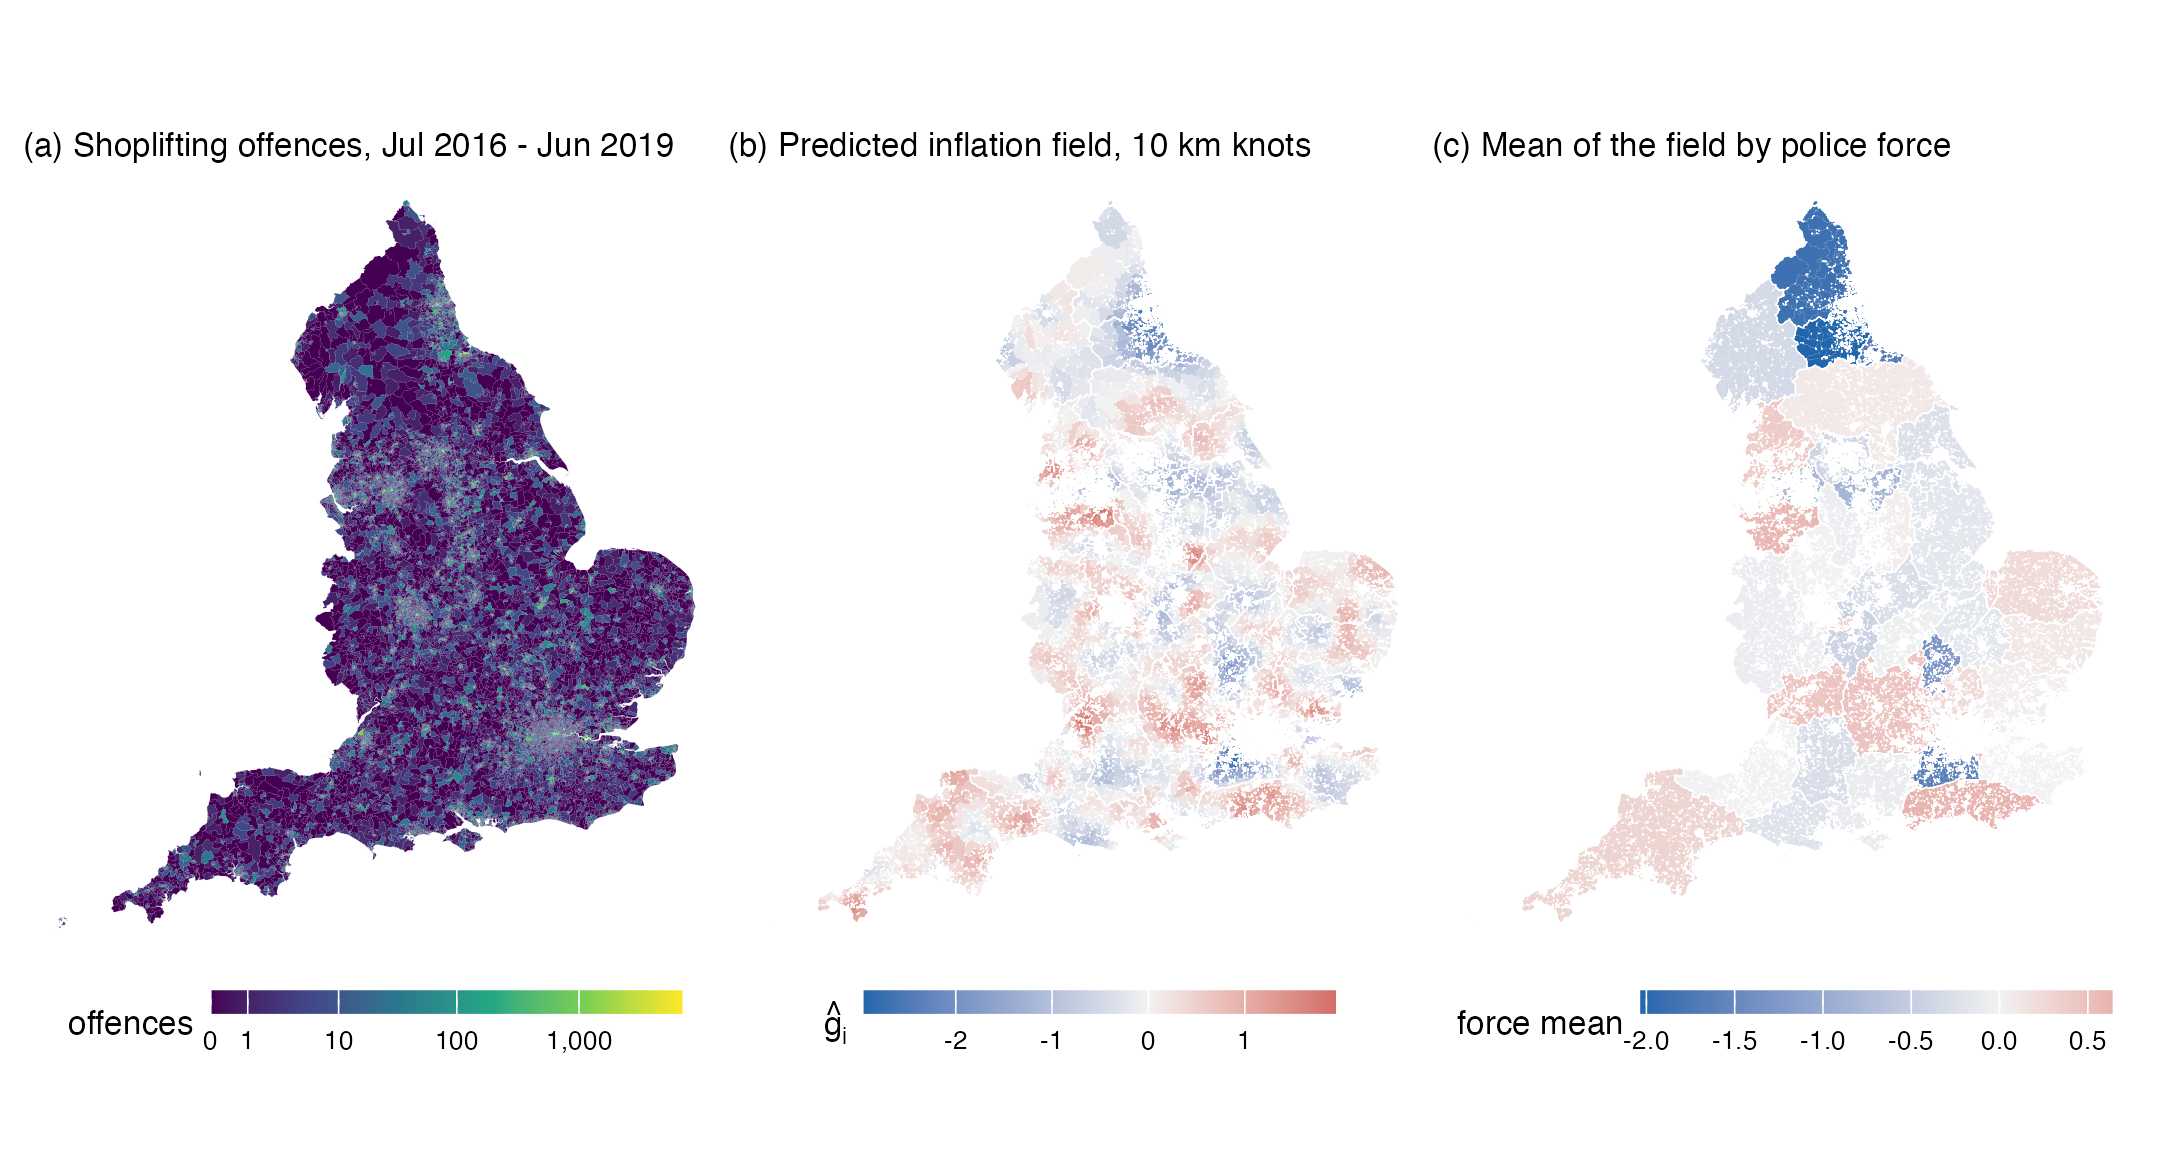
\includegraphics[width=\textwidth]{figures/crime_maps.png}
\caption{(a) Shoplifting offences recorded in each unit, July 2016--June 2019 (log scale). (b) Predicted inflation field $\hat g_i$ of the general ZISAR with knots 10~km apart; white lines are police force boundaries. (c) Mean of the field within each police force. A positive value raises the probability of a structural zero.}\label{fig:crime_maps}
\end{figure}

% ---------------------------------------------------------------------------
\subsection{What the field measures}\label{sec:crime_field}

Two readings are possible.
The field may capture retail that the BRES does not measure---owner-run shops, retail parks recorded under a neighbouring LSOA, market towns---in which case it describes the retail geography more finely than the covariates.
Or it may capture how offences are recorded: whether retailers report thefts, whether the force records them and where it locates them, which the inspection of crime data integrity by \citet{hmic2014} found to differ widely between forces.
The second reading has a testable implication: differences of recording are differences between forces, so fixed effects for the forces, in both processes, should absorb the field; differences in the unmeasured retail geography are not aligned with force boundaries and would not be.

The second column of Table~\ref{tab:crime_estimates} adds the 37 force indicators to both processes.
They raise the log-likelihood by 771 points (likelihood ratio 1{,}543 on 74 restrictions); the retail coefficients of the inflation process are unchanged ($-2.80$, $-1.28$ and $-0.12$ against $-3.13$, $-1.30$ and $-0.13$), while the count process reassigns to the forces part of what income deprivation and social renting were capturing.
The force effects of the two processes are distinct: those of the count process have a standard deviation of 0.28 and measure differences in the rate of recorded shoplifting; those of the inflation process are far larger and uncorrelated with them ($-0.07$), and for one force the effect diverges, no structural zero being attributed to it.
With the force effects the spatial structure of the zero regime disappears.
The score statistic falls to $-0.7$ null standard deviations over England and $-1.0$ outside London ($p = 0.74$ and $0.86$; London 1.2, $p = 0.11$); the profile of the reduced-rank field is flat (largest gain 4.3 points), and the fitted field has $\hat\rho_0 = 0$, a standard deviation of 0.21 and a likelihood ratio of 13: within a force, once the retail geography is accounted for, the structural zeros are not clustered.
The spatial structure of the zero regime is the structure of the police forces.

The field therefore identifies a regime of recording as much as a regime of absence.
Taken at face value, the structural zeros would describe where England has no shops; part of them describe instead where recorded shoplifting is absent because of how offences are reported and recorded, and these zeros cluster in space because forces cover contiguous territories.
A zero-inflated model of administrative counts cannot tell the two apart from the counts alone, but the inflation field tells the analyst where to look: the general ZISAR found the structure, the reduced-rank field made it estimable, and its geography pointed to the forces.
In administrative counts the zero regime is in part a property of the recording system, and a spatial field in the inflation process is the instrument for detecting it.
